\documentclass{report}
\usepackage[utf8]{inputenc}
\usepackage[T1]{fontenc}
\usepackage[francais]{babel}
\usepackage{titlesec}
\usepackage{amsmath}
\usepackage{amsfonts}
\usepackage{amssymb}
\usepackage{enumitem}
\usepackage{bbm}
\usepackage{hyperref}
\usepackage{fancyhdr}
\usepackage{stmaryrd}
\usepackage{ listings }
\usepackage{graphicx}
\usepackage{float}
\graphicspath{ {images/} }


\pagestyle{fancy}
%\usepackage[document]{ragged2e}


\DeclareMathOperator{\Tr}{Tr}
\DeclareMathOperator{\Id}{Id}
\DeclareMathOperator{\co}{co}
\DeclareMathOperator{\Ri}{Ri}
\DeclareMathOperator{\ext}{ext}


\begin{document}

\titleformat{\chapter}[display]
  {\normalfont\huge\bfseries\centering}
  {\chaptertitlename\ \thechapter}{10pt}{\Huge}

  \titleformat{\section}[block]
  {\normalfont\large\bfseries\centering}
  {\thesection}{3pt}{\large}

%\titleformat{\subsection}[runin]{\normalfont\large\bfseries\raggedleft}{\thesubsection}{0pt}{}



\renewcommand{\thesection}{\arabic{section}.}
\renewcommand{\thesubsection}{Exercice \arabic{section}.\arabic{subsection}}
\title{TD d'optimisation\\ ENSAE\\ 1A}
\author{Gabriel Romon}
\date{Version du \today}
\maketitle
\section{Différentielle}

\subsection{} \noindent\fbox{
\parbox{\linewidth}{
Soit $f:\mathbb R^2\to \mathbb R, (x,y)\mapsto \frac{x^3y^3}{x^2+y^2}$ si $(x,y)\neq (0,0)$ et $f(0,0)=0$.\newline
\begin{enumerate}[leftmargin=*]
\item Montrer que $f$ est $C^1$.
\item Montrer que $f$ est $C^2$.
\end{enumerate}
}}\\ 
\\ 
\\
\noindent 1. Les dérivées partielles de $f$ en $(x,y)\neq (0,0)$ sont clairement définies et données par $\frac{\partial f}{\partial x}(x,y)=\frac{x^2 y^3 \left(x^2+3 y^2\right)}{\left(x^2+y^2\right)^2}$ et $\frac{\partial f}{\partial y}(x,y)= \frac{x^3 y^2 \left(3 x^2+y^2\right)}{\left(x^2+y^2\right)^2}$. 
\newline
Comme pour tout $h\in \mathbb R, f(0,h)=f(h,0)=f(0,0)=0$, les dérivées partielles de $f$ existent en $(0,0)$ avec $\frac{\partial f}{\partial x}(0,0)=\frac{\partial f}{\partial y}(0,0)=0$.\newline
\newline
$(x,y)\mapsto \frac{\partial f}{\partial x}(x,y)$ et $(x,y)\mapsto \frac{\partial f}{\partial y}(x,y)$ sont clairement continues en tout $(x,y)\neq (0,0)$.
Montrons que ces deux fonctions sont continues en $(0,0)$.\newline
Pour $(x,y)\in \mathbb R^2$, si $x=0$ ou $y=0$, $\frac{\partial f}{\partial x}(x,y)=\frac{\partial f}{\partial y}(x,y)=0$. Dans la suite on supposera donc sans perte de généralité que $x\neq 0$ et $y\neq 0$.\newline
$\left| \frac{\partial f}{\partial x}(x,y)\right| =\left|\frac{x^2 y^3 \left(x^2+3 y^2\right)}{\left(x^2+y^2\right)^2}\right|\leq \frac{|y|^3x^4}{(x^2+y^2)^2} + 3\frac{|y|^5x^2}{(x^2+y^2)^2}\leq |y|^3+3|y|x^2 \xrightarrow[(x,y)\to (0,0)]{}0$\newline
$\left| \frac{\partial f}{\partial y}(x,y)\right| \leq |x|^3+3|x|y^2 \xrightarrow[(x,y)\to (0,0)]{}0$ par symétrie.\newline
$f$ admet donc des dérivées partielles qui sont définies et continues en tout point de $\mathbb R^2$. $f$ est donc $C^1$. \newline
\newline
2. $(x,y)\mapsto \frac{\partial f}{\partial x}(x,y)$ et $(x,y)\mapsto \frac{\partial f}{\partial y}(x,y)$ admettent clairement des dérivées partielles en tout $(x,y)\neq (0,0)$ données par $$\frac{\partial^2 f}{\partial x^2}(x,y)=-\frac{2 x y^5 \left(x^2-3 y^2\right)}{\left(x^2+y^2\right)^3}$$ $$\frac{\partial^2 f}{\partial yx}(x,y)=\frac{x^2 y^2 \left(3 x^4+14 x^2 y^2+3 y^4\right)}{\left(x^2+y^2\right)^3}$$ et par symétrie $$\frac{\partial^2 f}{\partial y^2}(x,y)=\frac{2 x^5 y \left(3 x^2-y^2\right)}{\left(x^2+y^2\right)^3}$$ $$\frac{\partial^2 f}{\partial xy}(x,y)=\frac{x^2 y^2 \left(3 x^4+14 x^2 y^2+3 y^4\right)}{\left(x^2+y^2\right)^3}$$
Comme pour tout $h\in \mathbb R$, $$\frac{\partial f}{\partial x}(0,h)=\frac{\partial f}{\partial x}(h,0)=\frac{\partial f}{\partial y}(0,h)=\frac{\partial f}{\partial y}(h,0)=\frac{\partial f}{\partial x}(0,0)=\frac{\partial f}{\partial y}(0,0)=0$$ les dérivées partielles de $\frac{\partial f}{\partial x}$ et  $\frac{\partial f}{\partial y}$ existent en $(0,0)$ avec $$\frac{\partial^2 f}{\partial x^2}(0,0)=\frac{\partial^2 f}{\partial y^2}(0,0)=\frac{\partial^2 f}{\partial xy}(0,0)=\frac{\partial^2 f}{\partial yx}(x,y)=0$$
\newline 
Les quatre dérivées partielles sont clairement continues en tout $(x,y)\neq (0,0)$. Montrons qu'elles sont continues en $(0,0)$. \newline
Soit $(x,y)\in \mathbb R^2$. Comme précédemment on peut supposer que $x\neq 0$ et $y\neq 0$.\newline
\newline
\textbf{Lemme}: $\forall (x,y)\in \mathbb R^2, |xy| \leq \|(x,y)\|_2^2$\newline
\underline{Preuve}: Conséquence de l'inégalité $ab\leq \frac{a^2+b^2}{2}$ avec $a=|x|$ et $b=|y|$.\newline
\newline
$$\begin{aligned}\left|\frac{\partial^2 f}{\partial x^2}(x,y)\right|&=\left|\frac{2 x y^5 \left(x^2-3 y^2\right)}{\left(x^2+y^2\right)^3}\right|\leq \frac{2|x|^3|y|^5}{(x^2+y^2)^3}+\frac{6|x||y|^7}{(x^2+y^2)^3}\\
&= \frac{2y^2 (|xy|)^3}{\|(x,y)\|_2^6} + \frac{6|x||y|^7}{(x^2+y^2)^3}\\
&{\leq} \underbrace{\frac{2y^2\|(x,y)\|_2^6}{\|(x,y)\|_2^6}}_{\text{Lemme}} + 6|x||y|\\
&=2y^2+ 6|x||y| \xrightarrow[(x,y)\to (0,0)]{}0
\end{aligned}$$
La symétrie permet de conclure $\left|\frac{\partial^2 f}{\partial x^2}(x,y)\right|\leq 2x^2+ 6|x||y| \xrightarrow[(x,y)\to (0,0)]{}0$ \newline et une technique similaire donne $$\left|\frac{\partial^2 f}{\partial yx}(x,y)\right|\leq 3y^2+ 14\|(x,y)\|_2^2+3x^2 \xrightarrow[(x,y)\to (0,0)]{}0$$
$\frac{\partial f}{\partial x}$ et $\frac{\partial f}{\partial y}$ admettent des dérivées partielles qui sont définies et continues en tout point de $\mathbb R^2$. Donc $f$ est $C^2$.

\subsection{} \noindent\fbox{
\parbox{\linewidth}{
Soit $f:\mathbb R^2\to \mathbb R, (x,y)\mapsto (x^2+y^2)^x$ si $(x,y)\neq (0,0)$.\newline
Montrer que $f$ est différentiable sur $\mathbb R^2\setminus \{(0,0)\}$.
}}\\ 
\\ 
\\
\noindent $f$ admet clairement des dérivées partielles en tout $(x,y)\neq (0,0)$ données par $\frac{\partial f}{\partial x}(x,y) = \left(x^2+y^2\right)^x \left(\frac{2 x^2}{x^2+y^2}+\log \left(x^2+y^2\right)\right)$ et $\frac{\partial f}{\partial y}(x,y) = 2 x y \left(x^2+y^2\right)^{x-1}$.\newline
Par composition et multiplication de fonction continues, ces dérivées partielles sont continues en tout $(x,y)\neq (0,0)$.\newline
$f$ est donc différentiable en tout $(x,y)\neq (0,0)$ et son gradient en $(x,y)$ est $$\left(\left(x^2+y^2\right)^x \left(\frac{2 x^2}{x^2+y^2}+\log \left(x^2+y^2\right)\right),2 x y \left(x^2+y^2\right)^{x-1}\right)$$

\subsection{} \noindent\fbox{
\parbox{\linewidth}{
Soit $f:\mathbb R^2\to \mathbb R^2, (x,y)\mapsto (x+y,xy)$.
Calculer la différentielle de $f$.
}}\\ 
\\ 
\\
\noindent Pour $(x,y)\in \mathbb R^2$ fixé et $(h_1,h_2)\in \mathbb R^2$, \newline 
$f((x,y)+(h_1,h_2))=f(x+h_1,y+h_2)=f(x,y)+\begin{pmatrix}
h_1+h_2 \\ yh_1 + xh_2
\end{pmatrix}^T + \begin{pmatrix}
0 \\ h_1 h_2
\end{pmatrix}^T$\newline
Le candidat pour la différentielle de $f$ en $(x,y)$ est donc $(h_1,h_2)\mapsto \left[\begin{pmatrix}
1 & 1\\
y & x 
\end{pmatrix} \begin{pmatrix}
h_1 \\ h_2
\end{pmatrix}\right]^T$. \newline
Il suffit de prouver que $\displaystyle \frac{\left\|(0,h_1h_2)\right\|}{\left\| 
(h_1, h_2)\right\|}\xrightarrow[\left\| 
(h_1, h_2)\right\|\to 0]{}0$\newline 
Le choix de la norme n'importe pas étant donné l'équivalence des normes en dimension finie. On choisit par exemple la norme $2$.\newline
$\displaystyle \frac{\left\|(0,h_1h_2)\right\|}{\left\| 
(h_1, h_2)\right\|} = \frac{|h_1 h_2|}{\sqrt{h^2_1+h^2_2}}\leq |h_1|\to 0$ \newline  en minorant trivialement le dénominateur par $\sqrt {h^2_2}$.

\subsection{} \noindent\fbox{
\parbox{\linewidth}{
Soit $f:M_n(\mathbb R) \to M_n(\mathbb R), X\mapsto X^TX$.
Calculer la différentielle de $f$.
}}\\ 
\\ 
\\
\noindent Pour $X\in M_n(\mathbb R)$ et $H\in M_n(\mathbb R)$, $f(X+H)=f(X)+X^TH+H^TX+H^TH$.\newline
Le candidat pour la différentielle de $f$ en $X$ est donc $H\mapsto X^TH+H^TX$.\newline
Il suffit de prouver que $\frac{\|H^TH\|}{\|H\|}\xrightarrow[\|H\|\to 0]{} 0$.\newline
Par équivalence des normes en dimension finie, on choisit n'importe quelle norme d'opérateur sur $M_n(\mathbb R)$ (celle qui dérive de la norme $2$ par exemple). Alors $\frac{\|H^TH\|}{\|H\|}\leq \frac{\|H^T\| \|H\|}{\|H\|} = \|H^T\|$. La transposée étant linéaire, elle est continue en $0$, donc $\|H^T\|\xrightarrow[\|H\|\to 0]{} 0 $ ce qui achève la preuve.

\subsection{} \noindent\fbox{
\parbox{\linewidth}{
Soient $f,g\in C^1(\mathbb R^2,\mathbb R)$ et $\varphi: \mathbb R^3\to \mathbb R^2, (x,y,z)\mapsto (f(x^2y,z^2x),g(x^y,zx))$\newline
Calculer, si elle existe, la différentielle de $f$.
}}\\ 
\\ 
\\
\noindent Posons $\gamma:(x,y,z)\mapsto (x^2y,z^2x)$ et $\delta:(x,y,z)\mapsto (x^y,zx)$.\newline
$\gamma$ et $f$ sont différentiables en tous points de leurs domaines, donc $f\circ \gamma$ est différentiable en tout point de $\mathbb R^3$ avec $$d(f\circ \gamma)(x,y,z) = df(\gamma(x,y,z))\circ d\gamma(x,y,z)$$
On calcule $\operatorname{Jac}(\gamma)(x,y,z)=\begin{pmatrix}
2xy & x^2 & 0 \\
z^2 & 0 & 2zx
\end{pmatrix}$.
En passant des applications linéaires aux matrices, $$\begin{aligned} \operatorname{Jac}(f\circ \gamma)(x,y,z) &= \operatorname{Jac}(f)(x^2y,z^2x)\cdot \operatorname{Jac}(\gamma)(x,y,z)\\
&= \operatorname{Jac}(f)(x^2y,z^2x) \cdot  \begin{pmatrix}
2xy & x^2 & 0 \\
z^2 & 0 & 2zx
\end{pmatrix} \end{aligned}$$\newline
$\delta$ est définie et différentiable en $(x,y,z)$ dès lors que $x>0$. On calcule de même $\operatorname{Jac}(\delta)(x,y,z)=\begin{pmatrix}
yx^{y-1} & x^y\ln x & 0 \\
z & 0 & x
\end{pmatrix}$ de sorte que pour tout $(x,y,z)$ avec $x>0$, $$ \operatorname{Jac}(g\circ \delta)(x,y,z)= \operatorname{Jac}(g)(x^y,zx) \cdot \begin{pmatrix}
yx^{y-1} & x^y\ln x & 0 \\
z & 0 & x
\end{pmatrix}$$
La différentielle de $f\circ \gamma$ en $(x,y,z)$ est donc $$\begin{pmatrix}
h_1 \\
h_2 \\
h_3
\end{pmatrix}^T \mapsto \left[\operatorname{Jac}(f)(x^2y,z^2x) \cdot  \begin{pmatrix}
2xy & x^2 & 0 \\
z^2 & 0 & 2zx
\end{pmatrix}\cdot \begin{pmatrix}
h_1 \\
h_2 \\
h_3
\end{pmatrix}\right]^T$$
et celle de $g\circ \delta$ en $(x,y,z)$ avec $x>0$
$$ \begin{pmatrix}
h_1 \\
h_2 \\
h_3
\end{pmatrix}^T \mapsto \left[\operatorname{Jac}(g)(x^y,zx) \cdot \begin{pmatrix}
yx^{y-1} & x^y\ln x & 0 \\
z & 0 & x
\end{pmatrix}\cdot \begin{pmatrix}
h_1 \\
h_2 \\
h_3
\end{pmatrix}\right]^T $$
Soit $(x,y,z)$ fixé avec $x>0$ et $h=(h_1,h_2,h_3)$ $$\begin{aligned} &\varphi\left( \begin{pmatrix} x \\y \\z \end{pmatrix} + \begin{pmatrix} h_1 \\ h_2 \\ h_3\end{pmatrix}\right) = \left( f\circ \gamma\left(\begin{pmatrix} x+h_1 \\y+h_2 \\z+h_3 \end{pmatrix}\right), g\circ \delta\left(\begin{pmatrix} x+h_1 \\y+h_2 \\z+h_3 \end{pmatrix}\right) \right)\\
&= (f\circ \gamma \left( (x,y,z)\right) + d(f\circ \gamma)\left(x,y,z\right) \left( h_1 , h_2 , h_3\right)+ ||h||\varepsilon_1(||h||),\\ 
&g\circ \delta \left( (x,y,z)\right) + d(g\circ \delta)\left(x,y,z\right) \left( h_1 , h_2 , h_3\right)+ ||h||\varepsilon_2(||h||)) \end{aligned}$$
où $\varepsilon_1$ et $\varepsilon_2$ sont des fonctions telles que $\varepsilon_1(||h||) \xrightarrow[||h||\to 0]{}0$ et $\varepsilon_2(||h||) \xrightarrow[||h||\to 0]{}0$
$$\begin{aligned}
=\varphi((x,y,z)) &+ (d(f\circ \gamma)\left(x,y,z\right) \left( h_1 , h_2 , h_3\right),d(g\circ \delta)\left(x,y,z\right) \left( h_1 , h_2 , h_3\right))\\
&+ ||h||\underbrace{(\varepsilon_1(||h||),\varepsilon_2(||h||))}_{\xrightarrow[||h||\to 0]{}0}
\end{aligned} $$
La différentielle de $\varphi$ en $(x,y,z)$ est donc 
$$\hspace{-2cm} \begin{pmatrix}
h_1 \\
h_2 \\
h_3
\end{pmatrix}^T \mapsto \left( \left[\operatorname{Jac}(f)(x^2y,z^2x) \cdot  \begin{pmatrix}
2xy & x^2 & 0 \\
z^2 & 0 & 2zx
\end{pmatrix}\cdot \begin{pmatrix}
h_1 \\
h_2 \\
h_3
\end{pmatrix}\right]^T, \left[\operatorname{Jac}(g)(x^y,zx) \cdot \begin{pmatrix}
yx^{y-1} & x^y\ln x & 0 \\
z & 0 & x
\end{pmatrix}\cdot \begin{pmatrix}
h_1 \\
h_2 \\
h_3
\end{pmatrix}\right]^T \right)$$

\subsection{} \noindent\fbox{
\parbox{\linewidth}{
Soit $E=C^0([a,b],\mathbb R)$ muni de la norme infinie $\|\cdot\|$ et $\varphi: E\to E, f \mapsto f^3$.\newline
Montrer que $\varphi$ est différentiable.
}}\\ 
\\ 
\\
\noindent On n'est plus dans le cadre des espaces de dimension finie et la notion de différentielle est celle de Fréchet.\newline
Pour $f\in E$ et $h\in E$, $\varphi(f+h) = \varphi(f) + 3f^2h + 3fh^2+h^3$.\newline
Le candidat pour la différentielle de $\varphi$ en $f$ est donc $h\mapsto 3f^2h $. \newline
Il suffit de prouver que $h\mapsto 3f^2h $ est continue en $0$ et que  $\frac{\| 3fh^2+h^3\|}{\|h \|} \xrightarrow[||h||\to 0]{}0$.\newline
\textbf{Lemme}: Pour $f,g\in E$, $\|fg\| \leq \|f\| \|g\|$.\newline
\underline{Preuve}: Par continuité de $|fg|$ sur $[a,b]$, il existe $c\in [a,b]$ tel que $$\|fg\| = |f(c)g(c)|\leq |f(c)| \|g\| \leq \|f\| \|g\|$$\\
\noindent D'après le lemme, $\|3f^2h \|\leq 3\|f^2\|\|h\|$ ce qui prouve la continuité en $0$.\newline
On a $\frac{\| 3fh^2+h^3\|}{\|h \|}\leq 3 \frac{\| f h^2\|}{\|h \|} + \frac{\|h^3 \|}{\|h \|}$.\newline
Le lemme donne $\frac{\| 3fh^2+h^3\|}{\|h \|}\leq 3\|f\| \|h\| + \|h\|\xrightarrow[||h||\to 0]{}0$.

\subsection{} \noindent\fbox{
\parbox{\linewidth}{
Soit $E=C^0([0,1],\mathbb R)$ muni de la norme infinie $\|\cdot\|$ et $g:\mathbb R\to \mathbb R$ deux fois dérivable avec $g''$ bornée par $M\geq 0$.\newline
Soit $I:E\to \mathbb R, f\mapsto \int_0^1 (g\circ f)(t) dt$
\begin{enumerate}[leftmargin=*]
\item Montrer que $I$ est différentiable et calculer sa différentielle.
\item Montrer que $I$ est $C^1$.
\item Qu'en est-il si $g$ est seulement $C^1$?
\end{enumerate}
}}\\ 
\\ 
\\
\noindent 1. Pour $f\in E$ fixé et $h\in E$, $t\in [0,1]$, la formule de Taylor-Lagrange donne $$g(f(t)+h(t))=g(f(t))+h(t)g'(t)+\frac{h(t)^2}{2}g''(\xi_{h,t})$$ où $\xi_t\in \mathbb R$ de sorte que $t\mapsto \frac{h(t)^2}{2}g''(\xi_{h,t})$ est continue sur $[0,1]$ et $$I(f+h) = I(f) + \int_0^1 h(t)g'(f(t)) dt + \int_0^1 \frac{h(t)^2}{2}g''(\xi_{h,t}) dt$$ 
Le candidat pour la différentielle de $I$ en $f$ est $h\mapsto \int_0^1 h(t)g'(f(t)) dt$. \newline
Il suffit de prouver que $h\mapsto \int_0^1 h(t)g'(f(t)) dt$ est continue en $0$ et $$\frac{\left|\int_0^1 \frac{h(t)^2}{2}g''(\xi_{h,t}) dt\right|}{\|h\|}\xrightarrow[||h||\to 0]{}0$$
On a $\left|\int_0^1 h(t)g'(f(t)) dt\right|\leq \|h\|\underbrace{\int_0^1|g'(f(t))|dt}_{\text{indépendant de }h}$ ce qui prouve la continuité en $0$.\newline
Comme $\left|\frac{h(t)^2}{2}g''(\xi_{h,t}) \right|\leq \frac{M}{2} h(t)^2$, $$\frac{\left|\int_0^1 \frac{h(t)^2}{2}g''(\xi_{h,t}) dt\right|}{\|h\|}\leq \frac{M}{2} \frac{\int_0^1 h(t)^2 dt}{\|h\|}\leq \frac{M}{2} \frac{\|h\|^2}{\|h\|}= \frac{M}{2}\|h\|\xrightarrow[||h||\to 0]{}0$$
2. Sur $\mathcal L_c(E,\mathbb R)$ on institue la norme d'opérateur $\|\cdot \|_{op}$ dérivant de la norme infinie.\newline
Il s'agit de montrer la continuité de $\varphi: 
\begin{cases}
      E & \longrightarrow \; \mathcal L_c(E,\mathbb R) \\
      f & \longmapsto \; \begin{cases} E &  \longrightarrow \; \mathbb R \\ h & \longmapsto \; \int_0^1 h(t)g'(f(t))dt \end{cases}
    \end{cases}
$\newline
Soit $f_0\in E$ et $h\in E$. On a $$\begin{aligned}|\varphi(f)(h)-\varphi(f_0)(h)|&=\left|\int_0^1 h(t)(g'(f(t))-g'(f_0(t))) \right|\\
&\leq \int_0^1 |h(t)| M |f(t)-f_0(t)| dt \quad g''\text{ est bornée par }M\text{ donc }g' \text{ est } M\text{-lipschitzienne}\\
&\leq M\|f-f_0\|\int_0^1 |h(t)| dt \\
&\leq M\|f-f_0\| \|h\|
\end{aligned}$$
Donc $\frac{|\varphi(f)(h)-\varphi(f_0)(h)|}{\|h\|}$ est bornée par $M\|f-f_0\|$, d'où $$ \| \varphi(f) - \varphi (f_0)\|_{op} = \sup_{h} \frac{|\varphi(f)(h)-\varphi(f_0)(h)|}{\|h\|}\leq M\|f-f_0\| $$
Soit $\varepsilon>0$. Avec $\delta := \frac{\varepsilon}{M}$, $\|f-f_0\|\leq \delta \implies \| \varphi(f) - \varphi (f_0)\|_{op} \leq \varepsilon $\newline
 ce qui prouve la continuité de $\varphi$ en $f_0$.\newline
3. Mon intuition me laisse penser que si $g$ est deux fois dérivable sans être bornée (donc $C^1$), $I$ n'est pas forcément différentiable. Obtenir un contre-exemple n'est pas évident, car $I$ est tout de même continue (par uniforme continuité de $g$ sur un compact).

\subsection{} \noindent\fbox{
\parbox{\linewidth}{
Soient $E$ et $F$ des evn avec $F$ complet. Soit $D\subset E$ un ouvert.\newline
On pose $B^2=\{ f:D\to F/\; f \; C^2, f\text{ bornée, } df\text{ bornée, et } d^2f \text{ bornée} \}$ et \newline
$$\|f\| = \sup_{x\in D}( \|f(x)\| + \|df(x)\| + \|d^2f(x)\|)$$ 
Montrer que $B^2$ est complet.
}}\\ 
\\ 
\\
\noindent On trouvera une présentation de l'intégrale des fonctions à valeurs dans un espace de Banach à l'adresse \newline  \url{http://www.math.ucsd.edu/~bdriver/231-02-03/Lecture_Notes/chap4.pdf} \newline \newline 
Etant donné $X$ un ensemble et $(Y,\|\cdot\|_Y)$ un evn, on note $B(X,Y)$ l'ensemble des fonctions bornées de $X$ dans $Y$. On rappelle que si $Y$ est complet, alors $B(X,Y)$ est complet pour la norme $\|\cdot\|_{\infty,Y}$ définie par $\|f\|_{\infty,Y}=\sup_{x\in X}\|f(x)\|_Y$.\newline \newline
On notera $\|\cdot\|_{op}$ la norme d'opérateur sur $\mathcal L_c(E,F)$ qui dérive de $\|\cdot\|_F$. On rappelle que $(\mathcal L_c(E,F),\|\cdot\|_{op})$ est un Banach.\newline \newline
On notera $\|\cdot\|_{op'}$ la norme d'opérateur sur $\mathcal L_c(E,\mathcal L_c(E,F))$ qui dérive de $\|\cdot\|_{op}$, de sorte que $(\mathcal L_c(E,\mathcal L_c(E,F)),\|\cdot\|_{op'})$ est un Banach.\newline \newline
On rappelle que si $f\in B^2$ et $a\in D$, $df(a)\in \mathcal L_c(E,F)$ et $d^2f(a) \in \mathcal L_c(E,\mathcal L_c(E,F))$. La norme définie dans l'énoncé est donc à prendre au sens suivant: $$\|f\| = \sup_{x\in D}( \|f(x)\|_F + \|df(x)\|_{op} + \|d^2f(x)\|_{op'})$$ 
On prouve facilement les faits suivants: pour $f\in B^2$, \newline
$\|f\|\geq \|f\|_{\infty, F}$ \newline
$\|f\|\geq \|df\|_{\infty, op}$ \newline
$\|f\|\geq \|d^2f\|_{\infty, op'}$ \newline 
\newline
Soit $(f_n)$ de Cauchy dans $B^2$ pour $\|\cdot \|$.\newline
$\bullet$ D'après la remarque précédente, $(f_n)$ est de Cauchy pour $\|\cdot\|_{\infty, F}$ dans $B(D,F)$ qui est complet, donc $(f_n)$ converge pour $\|\cdot\|_{\infty, F}$ vers un $f\in B(D,F)$.\newline
$\bullet$ D'après la remarque précédente, $(df_n)$ est de Cauchy pour $\|\cdot\|_{\infty, op}$ dans $B(D,\mathcal L_c(E,F))$ qui est complet, donc $(df_n)$ converge pour $\|\cdot\|_{\infty, op}$ vers un $\varphi\in B(D,\mathcal L_c(E,F))$.\newline
$\bullet$ En tant que limites uniformes de fonctions continues, $f$ et $\varphi$ sont continues.\newline
$\bullet$ Montrons que $f$ est différentiable de différentielle $\varphi$.\newline
Soit $a\in D$. Pour $h\in D$, et $n$ quelconque, $$f_n(a+h)-f_n(a)=\int_0^1 df_n(a+th)dt$$
La convergence des $df_n$ vers $\varphi$ étant uniforme, on a en passant à la limite $$f(a+h)-f(a) = \int_0^1 \varphi(a+th) dt$$
donc $$\begin{aligned} \frac{\|f(a+h)-f(a)-\varphi(a)(h)\|_F}{\|h\|_E}&=\frac{\|\int_0^1 \varphi(a+th)-  \varphi(a)(h) dt\|_F}{\|h\|_E} \\
&\leq \frac{\int_0^1 \|\varphi(a+th)-\varphi(a)\|_{op}\|h\|_E dt}{\|h\|_E}\\
&\leq \int_0^1 \|\varphi(a+th)-\varphi(a)\|_{op} dt \end{aligned}$$
Soit $\varepsilon>0$. Comme $\varphi$ est continue on dispose de $\delta >0$ tel que $\|x\|_F \leq \delta \implies \|\varphi(a+x)-\varphi(a)\|_{op} \leq \varepsilon$. Pour $\|h\| \leq \varepsilon$ et $t\in [0,1]$ on obtient $$\|\varphi(a+th)-\varphi(a)\|_{op}\leq \varepsilon$$ donc $\displaystyle \frac{\|f(a+h)-f(a)-\varphi(a)(h)\|_F}{\|h\|_E}\leq \varepsilon$ dès que $\|h\| \leq \delta$.\newline
$f$ est donc différentiable sur $D$ et sa différentielle est $\varphi$, qui est continue d'après la remarque précédente.\newline
$\bullet$ Un raisonnement identique en remplaçant $f_n$ par $df_n$ montre que $df$ est différentiable sur $D$, on note $d^2f$ sa différentielle qui est continue.\newline
$\bullet$ $f$ est donc $C^2$, bornée, de différentielles bornées. Il reste à prouver que $(f_n)$ converge vers $f$ pour la norme $\|\cdot\|$.\newline
Etant donné $\varepsilon >0$, on dispose de $N,N',N''$ tels que $$ 
\forall x\in D, \begin{array}[t]{lcl} n\geq N &\implies &\|f(x) -f_n(x)\|_F \leq \frac{\varepsilon}3 \\
n\geq N' &\implies &\|df(x) -df_n(x)\|_{op} \leq \frac{\varepsilon}3 \\
n\geq N'' &\implies &\|d^2f(x) -df^2_n(x)\|_{op'} \leq \frac{\varepsilon}3
\end{array}$$
Pour $n\geq \max(N,N',N'')$, $$\|f(x) -f_n(x)\|_F+\|df(x) -df_n(x)\|_{op}+\|d^2f(x) -df^2_n(x)\|_{op'}\leq \varepsilon$$ et ceci pour tout $x\in D$, donc $\|f-f_n\|\leq \varepsilon$. Ceci achève la preuve.

\subsection{} \noindent\fbox{
\parbox{\linewidth}{
Soit $E$ un $\mathbb R$-evn, $D\subset E$ un ouvert et $f:\overline{D}\to \mathbb R$. On suppose $\overline{D}$ compact, $f$ continue, nulle à la frontière de $D$ et $f$ différentiable sur $D$.\newline
Montrer qu'il existe $a\in D$ tel que $df(a)=0$.
}}\\ 
\\ 
\\
\noindent $f$ est continue sur le compact $\overline D$ donc elle admet un maximum $M$ et un maximum $m$ atteints respectivement en $\alpha$ et $\beta \in \overline D$.\newline
Si $m=M=0$, $f$ est nulle sur $D$ donc pour tout $x\in D$, $df(x)=0$.\newline
Sinon, $m<0$ ou $M>0$. On suppose par exemple $M>0$. Comme $f$ est nulle sur $\overline D\setminus \mathring D = \overline D\setminus D$, on a $\beta \in D$. En $\beta$, $f$ admet un maximum global (donc local), d'où $df(\beta)=0$. 

\subsection{} \noindent\fbox{
\parbox{\linewidth}{
Soient $\varphi,\psi\in C^1(\mathbb R, \mathbb R)$ et $f(x,y,z)=(x+\varphi(yz),y+\psi(\frac xz))$.\newline
Calculer la différentielle de $f$.
}}\\ 
\\ 
\\
\noindent La démarche est identique à celle de l'exercice 1.5. En posant $f_1:(x,y,z)\mapsto x+\varphi(yz)$ et $f_2:(x,y,z)\mapsto y+\psi(\frac xz)$, il suffit de démontrer que $f_1$ et $f_2$ sont différentiables en $(x,y,z)$ pour obtenir la différentielle de $f$ en $(x,y,z)$: $$df(x,y,z):(h_1,h_2,h_3)\mapsto (df_1(x,y,z)(h_1,h_2,h_3),df_2(x,y,z)(h_1,h_2,h_3))$$
On calcule $$\operatorname{Jac}(f_1)(x,y,z)=(1,\varphi'(yz)z,\varphi'(yz)y)$$ et $$\operatorname{Jac}(f_2)(x,y,z)=\left(\psi(\frac xz)\frac 1z,1,-\psi(\frac xz) \frac{x}{z^2} \right)$$


\subsection{} \noindent\fbox{
\parbox{\linewidth}{
\begin{enumerate}[leftmargin=*]
\item Soient $E,F,G,H$ des $\mathbb R$-evn. $B$ est une forme bilinéaire continue de $F\times G$ dans $H$, $f:E\to F$ et $g:E\to G$.\newline
On suppose que $f$ et $g$ sont différentiables en $a\in E$. Montrer que $C:E\to H, x\mapsto B(f(x),g(x))$ est différentiable en $a$.
\item Soit $E$ un espace vectoriel euclidien.
\begin{enumerate}
\item Montrer que $\varphi:x\mapsto \frac{x}{\|x\|^2}$ est différentiable sur $E\setminus \{0\}$.
\item Déterminer la différentielle de $\psi:x \mapsto \|x\|^2$.
\item Déterminer et interpréter la différentielle de $\varphi$.
\end{enumerate}

\end{enumerate}
}}\\ 
\\ 
\\
\noindent 1. Soit $a\in E$. Pour $h\in E$, 
$$\begin{aligned}C(a+h)=&C(a) + B(f(a),dg(a)(h)) + B(df(a)(h),g(a))\\
&+ \\
&B(f(a),\|h\|\varepsilon_g(\|h\|)) + B(df(a)(h), dg(a)(h)+\|h\|\varepsilon_g(\|h\|)) + B(\|h\|\varepsilon_f(\|h\|),g(a+h))
\end{aligned}$$
Le candidat pour la différentielle en $a$ de $f$ est $h\mapsto B(f(a),dg(a)(h)) + B(df(a)(h),g(a))$.\newline
Il suffit de prouver que $$B(f(a),\|h\|\varepsilon_g(\|h\|)) + B(df(a)(h), dg(a)(h)+\|h\|\varepsilon_g(\|h\|)) + B(\|h\|\varepsilon_f(\|h\|),g(a+h)) = o(\|h\|)$$
$B$ étant bilinéaire continue, il existe $K\geq 0$ tel que $$\forall x,y\in E, \|B(x,y)\|\leq K \|x\| \|y\|$$
On traite chaque terme de la somme séparément: \newline
$\bullet$ $B(f(a),\|h\|\varepsilon_g(\|h\|))=\|h\|\underbrace{B(f(a),\varepsilon_g(\|h\|))}_{\to 0}$\newline\newline
$\bullet$ $\|B(df(a)(h), dg(a)(h))\|\leq K \|df(a)\|_{op}\|df(b)\|_{op} \|h\|^2$ \newline\newline
$\bullet$ $B(df(a)(h),\|h\|\varepsilon_g(\|h\|)) =\|h\| \underbrace{B(df(a)(h),\varepsilon_g(\|h\|))}_{\to 0} $\newline\newline
$\bullet$ $B(\|h\|\varepsilon_f(\|h\|),g(a+h)) =\|h\| \underbrace{B(\varepsilon_f(\|h\|),g(a+h))}_{\to 0}$\newline \newline
La somme est bien $o(\|h\|)$.\newline \newline 
2. a) $(x,y)\mapsto\langle x,y \rangle$ est bilinéaire continue (d'après Cauchy-Schwarz). La question 1. implique que $\psi:x\mapsto \langle x,x \rangle$ est différentiable en tout $a\in  E$. La fonction $\delta: x\mapsto \frac 1x$ est différentiable en tout $a\in \mathbb R\setminus \{0\}$ donc $\delta\circ \psi$ est différentiable en tout $a\in E\setminus \{0\}$.\newline
$\pi: \mathbb R\times E \to  E,\; (\lambda,x)\mapsto \lambda x$ est bilinéaire continue, et d'après 1., $x\mapsto \pi(\delta\circ \psi(x),x)$ est différentiable en tout $x\in E\setminus \{0\}$.\newline
Ceci s'écrit encore $\varphi:x\mapsto \frac{x}{\|x\|^2}$ est différentiable sur $E\setminus \{0\}$. \newline 
\newline
b) Soit $x\in E$. Pour $h\in E$, $\psi(x+h)= \psi(x) + 2\langle x,h \rangle + \|h\|^2$. \newline
La différentielle de $\psi$ en $x$ est donc $h\mapsto 2\langle x,h \rangle$.\newline
\newline
c) D'après 1., la différentielle de $\varphi$ en $x\neq 0$ est donnée par $$ \begin{aligned} d\varphi(x)(h)&= \pi(\Id(x),d(\delta\circ \psi)(x)(h)) +\pi(d\Id(x)(h),\delta\circ \psi(x))\\
&= x\cdot d\delta(\psi(x))(d\psi(x)(h)) + \frac{h}{\|x\|^2}\\
&= x\cdot -\frac{2\langle x,h\rangle}{(\|x\|^2)^2} + \frac{h}{\|x\|^2}\\
&= \frac{h}{\|x\|^2} - \frac{2\langle x,h\rangle x}{\|x\|^4} \end{aligned}$$

\subsection{} \noindent\fbox{
\parbox{\linewidth}{
Déterminer toutes les fonctions $f\in C^2(\mathbb R^2,\mathbb R)$ telles que $$\frac{\partial^2f}{\partial x^2}=\frac{\partial^2f}{\partial y^2}$$
}}\\ 
\\ 
\\
\noindent C'est un classique que l'on trouve dans n'importe quel livre de prépa.

\subsection{} \noindent\fbox{
\parbox{\linewidth}{
En quels points de $\mathbb R^2$ la fonction $g:(x,y)\mapsto \max(x^2,y)$ est-elle différentiable ? Calculer sa différentielle.
}}\\ 
\\ 
\\
\noindent Soit $(x,y)\in \mathbb R^2$ tel que $x^2>y$. Cette relation reste vérifiée sur un voisinage de $(x,y)$ de sorte que $g(x,y)=x^2$ sur un voisinage de $(x,y)$. $g$ est donc différentiable en $(x,y)$ de différentielle $(h_1,h_2)\mapsto 2xh_1$.\newline \newline
Soit $(x,y)\in \mathbb R^2$ tel que $x^2<y$. Cette relation reste vérifiée sur un voisinage de $(x,y)$ de sorte que $g(x,y)=y$ sur un voisinage de $(x,y)$
$g$ est donc différentiable en $(x,y)$ de différentielle $(h_1,h_2)\mapsto h_2$.\newline \newline
En $(0,0)$: $\displaystyle \frac{g(0,\frac 1n) - g(0,0)}{\frac 1n} = 1$ et $\displaystyle \frac{g(0,-\frac 1n) - g(0,0)}{-\frac 1n}=0$ donc $g$ n'admet pas de dérivée partielle selon $y$ en $(0,0)$ donc $g$ n'est pas différentiable en $(0,0)$. \newline \newline
Soit $(x,y)\in \mathbb R^2$ avec $x^2=y$ et $x\neq 0$. $$\displaystyle \frac{g(x+\frac 1n,y) - g(x,y)}{\frac 1n} = \frac{\left(x+\frac 1n \right)^2-x^2}{\frac 1n}\xrightarrow[n\to \infty]{} 2x$$
$$\displaystyle \frac{g(x-\frac 1n,y) - g(x,y)}{-\frac 1n} = \frac{y-y}{-\frac 1n}=0\neq 2x$$
donc $g$ n'admet pas de dérivée partielle selon $x$ en $(x,y)$ donc $g$ n'est pas différentiable en $(x,y)$.

\subsection{} \noindent\fbox{
\parbox{\linewidth}{
Soient $n\geq 1$ et $p\geq 1$ des entiers. \newline On définit $\displaystyle f:\mathbb R^2\to \mathbb R, (x,y)\mapsto \frac{x^ny^p}{x^2+y^2}$ si $(x,y)\neq (0,0)$ et $f(0,0)=0$. \newline
Pour quelles valeurs de $(n,p)$ $f$ est-elle différentiable dans $\mathbb R^2$ ?
}}\\ 
\\ 
\\
\noindent Quelles que soient les valeurs de $n$ et $p$, $f$ est différentiable en $(x,y)\neq (0,0)$ par composition. $f$ admet donc des dérivées partielles données par $$\frac{\partial f}{\partial x}(x,y) = \frac{n x^{n-1} y^p}{x^2+y^2}-\frac{2 x^{n+1} y^p}{\left(x^2+y^2\right)^2}$$ et $$\frac{\partial f}{\partial y}(x,y)=\frac{p x^n y^{p-1}}{x^2+y^2}-\frac{2 x^n y^{p+1}}{\left(x^2+y^2\right)^2}$$ \newline
En $(0,0)$: comme pour tout $h\in \mathbb R, f(0,h)=f(h,0)=f(0,0)=0$, les dérivées partielles de $f$ existent en $(0,0)$ avec $\frac{\partial f}{\partial x}(0,0)=\frac{\partial f}{\partial y}(0,0)=0$.\newline \newline 
On étudie plusieurs cas selon $n$ et $p$. Si les dérivées partielles sont continues en $(0,0)$, $f$ est différentiable en $(0,0)$. Si ce n'est le pas on ne peut a priori rien dire.\newline
On utilise les mêmes techniques de majoration que dans l'exercice 1.
\begin{enumerate}
\item Si $n\geq 4$: OK 
\item Si $n=3$: \begin{enumerate}
\item Si $p\geq 4$: OK par symétrie
\item Si $p=3$: OK 
\item Si $p=2$: OK
\item Si $p=1$: OK
\end{enumerate}
\item Si $n=2$: \begin{enumerate}
\item Si $p\geq 4$: OK par symétrie
\item Si $p=3$: OK par symétrie
\item Si $p=2$: OK
\item Si $p=1$: Pour $t\in \mathbb R$ non nul, $$ \frac{f\left((0,0)+t(1,1)\right) - f((0,0))}{t} = \frac 12$$
$f$ admet donc une dérivée directionnelle selon le vecteur $(1,1)$ qui vaut $\frac 12$.\newline
Si $f$ était différentiable en $(0,0)$, son gradient donné par les dérivées partielles serait nul, donc la différentielle en $(0,0)$ serait aussi nulle, donc toutes les dérivées directionnelles seraient aussi nulles, ce qui n'est pas le cas. $f$ n'est donc pas différentiable en $(0,0)$.
\end{enumerate}
\item Si $n=1$: \begin{enumerate}
\item Si $p\geq 4$: OK par symétrie
\item Si $p=3$: OK par symétrie
\item Si $p=2$: Non par symétrie
\item Si $p=1$: $f(0,\frac{1}{n})=0$ et $f(\frac{1}{n},\frac{1}{n})=\frac{1}{2}$, donc $f$ n'est pas continue en $0$, donc pas différentiable en $(0,0)$.
\end{enumerate}
\end{enumerate}
\textbf{Conclusion}: $f$ est différentiable en $(0,0)$ pour tout $n\geq 1$ et $p\geq 1$ exceptés les couples $(n=2,p=1),(n=1,p=2),(n=1,p=1)$.
\subsection{} \noindent\fbox{
\parbox{\linewidth}{
Soit $B$ dans $M_n(\mathbb R)$.\newline
Donner la différentielle de $\varphi: GL_n(\mathbb R) \to \mathbb R, A\mapsto \Tr(A^{-1}B)$
}}\\ 
\\ 
\\
\noindent On choisit une norme d'opérateur $\| \cdot \|$ sur $M_n(\mathbb R)$. On rappelle que $GL_n(\mathbb R)$ est ouvert.\newline
Soit $A\in GL_n(\mathbb R)$. On considère $V\subset GL_n(\mathbb R)$ un voisinage de $A$ tel que pour tout $X\in V$, $\|A^{-1}(X-A)\| <1$. Calculons la différentielle de la fonction $M\to M^{-1}$ en $A$.\newline
Il existe $\delta>0$ tel que pour tout $H\in M_n(\mathbb R)$, $\|H\| \leq \delta \implies A+H\in V$.\newline
Pour $\|H\|\leq \delta$, $(A+H)^{-1}=(I_n+A^{-1}H)^{-1}A^{-1}$.\newline
Démontrons que $(I_n+A^{-1}H)^{-1} = \sum_{k=0}^\infty (-1)^k (A^{-1}H)^k$. Comme $\|H\|\leq \delta$, $\|A^{-1}H\| <1$ donc la série en question est absolument convergente, donc convergente. On a pour $N\geq 1$, $$(I_n+A^{-1}H)\sum_{k=0}^N (-1)^k (A^{-1}H)^k = (-1)^N\underbrace{(A^{-1}H)^{N+1}}_{\xrightarrow[N\to \infty]{}0} + I_n$$
En passant à la limite sur $N$ on a l'égalité voulue. \newline
Par conséquent $$(A+H)^{-1}= \sum_{k=0}^\infty (-1)^k (A^{-1}H)^kA^{-1}=A^{-1} - A^{-1}HA^{-1}+\sum_{k=2}^\infty (-1)^k (A^{-1}H)^kA^{-1}$$
La candidat pour la différentielle de l'inverse en $A$ est donc $H\mapsto - A^{-1}HA^{-1}$.\newline
Il reste à remarquer que $$ \frac{\| \sum_{k=2}^\infty (-1)^k (A^{-1}H)^kA^{-1} \|}{\| H\|}\leq \frac{\|A^{-1}\|^2}{1-\|A^{-1}H\|}\|H\|\to 0$$
La fonction $A\mapsto \Tr(AB)$ étant linéaire, la différentielle de $\varphi$ en $A$ est donnée par $H\mapsto -\Tr(A^{-1}HA^{-1}B)$

\subsection{} \noindent\fbox{
\parbox{\linewidth}{
Soit $\varphi: \mathbb R \to GL_n(\mathbb R), x\mapsto A(x)$\newline
Calculer la différentielle de $x\mapsto \ln \det A(x)$
}}\\ 
\\ 
\\
\noindent Il est classique (cf Gourdon Analyse ou Cassini Algèbre 2) que la différentielle du déterminant en $A$ est donnée par $H\mapsto \Tr((\operatorname{com} A)^TH)$ qui devient $H\mapsto \det A \Tr(A^{-1}H)$ lorsque $A$ est inversible.\newline 
Pour $a\in \mathbb R$ et $h\in \mathbb R$, $$\begin{aligned} 
d(\ln \circ \det \circ A)(a)(h) &= d(\ln \circ \det)(A(a))(dA(a)(h))\\
&= h \cdot d(\ln \circ \det)(A(a))(dA(a)(1)) \\
&= h \cdot d(\ln \circ \det)(A(a))( \frac{dA}{dx}(a) ) \\
&= h \cdot d\ln (\det A(a))\left( d\det (A(a))(\frac{dA}{dx}(a)) \right) \\
&= h \cdot d\ln (\det A(a))\left ( \det A(a) \Tr\left (A(a)^{-1}\frac{dA}{dx}(a)\right) \right)  \\
&= h \det A(a) \Tr\left (A(a)^{-1}\frac{dA}{dx}(a)\right) d\ln (\det A(a))(1) \\
&= h \Tr\left (A(a)^{-1}\frac{dA}{dx}(a)\right)
\end{aligned}$$
La différentielle cherchée en $a$ est donc $h\mapsto h \Tr\left (A(a)^{-1}\frac{dA}{dx}(a)\right)$

\subsection{} \noindent\fbox{
\parbox{\linewidth}{
Soient $f$ et $g$ deux fonctions $\mathbb R \to \mathbb R$ dérivables en $1$. Montrer que $\varphi:(x,y)\mapsto f(xy)+g(\frac{x}{y})$ est différentiable en $(1,1)$ et calculer sa différentielle en $(1,1)$.
}}\\ 
\\ 
\\
\noindent Soient $\alpha:\mathbb R^2\to \mathbb R, (x,y)\mapsto xy$ et $\beta:\mathbb R\times \mathbb R\setminus\{0\} \to \mathbb R, (x,y)\mapsto \frac{x}{y}$.\newline
On dispose de $U$ un voisinage de $(1,1)$ et $V$ un voisinage de $1$ tel que $\alpha(U)\subset V$ et $\beta(U)\subset V$. $\alpha:U\to V$ et $\beta:U \to V$ sont différentiables en $(1,1)$.\newline 
 Le théorème de composition s'applique: $f\circ \alpha$ et $f\circ \beta$ sont différentiables en $(1,1)$, donc $\varphi$ aussi, avec 
 $$\begin{aligned} d\varphi((1,1))(h_1,h_2) &= d(f\circ \alpha)(1,1)(h_1,h_2)+d(f\circ \beta)(1,1)(h_1,h_2)\\
 &= (yh_1+xh_2)f'(1) + (-\frac{y}{x^2}h_1+\frac{h_2}{x})g'(1)
 \end{aligned}$$

\subsection{} \noindent\fbox{
\parbox{\linewidth}{
Déterminer toutes les fonctions $f$ de classe $C^2$ sur $\mathbb R\setminus \{-1,1\}$ qui vérifient $\frac{\partial^2 Z}{\partial x^2}-\frac{\partial^2 Z}{\partial y^2}=\frac{y}{x^3}$ où $Z(x,y)=f(\frac{y}{x})$
}}\\ 
\\ 
\\
\noindent ?


 \subsection{} \noindent\fbox{
\parbox{\linewidth}{
Soient $E$ et $F$ deux espaces de Banach. Soit $f:E\to F$ de classe $C^2$ telle que $$\forall t \in \mathbb R, \forall x\in E, f(tx)=t^2f(x)$$
Montrer que pour tout $x\in E$, $d^2f(0)(x,x)=2f(x)$.
}}\\ 
\\ 
\\
\noindent On rappelle que $\mathcal L_c(E,\mathcal L_c(E,F))$ s'identifie à l'espace des applications bilinéaires $\mathcal L_c(E\times E, F)$.\newline
L'énoncé demande en réalité de montrer que pour tout $x\in E$, $$d^2f(0)(x)(x)=2f(x)$$
Soit $x\in E$ fixé. \newline 
Posons $\alpha:\mathbb R\to E, t\mapsto tx$ et $\beta: \mathbb R\to F, t\mapsto t^2f(x)$. $\mathbb R$ étant de dimension finie, toute application linéaire de $\mathbb R$ dans $E$ est continue. $\alpha$ est clairement différentiable en tout $t\in \mathbb R$ de différentielle $h\mapsto hx$.\newline 
Pour $t\in \mathbb R$ et $h\in \mathbb R$, $\beta(t+h)=\beta(t)+2thf(x)+h^2f(x)$ avec $$\frac{\|h^2f(x)\|_F}{|h|}=|h|\|f(x)\|_F \xrightarrow[|h|\to 0]{}0 $$
Donc $\beta$ est différentiable en $t$ de différentielle $h\mapsto 2thf(x) $ \newline \newline
En différentiant l'égalité $f\circ \alpha =\beta $ en $t\in \mathbb R$ on a pour tout $h\in \mathbb R$, $hdf(tx)(x)=2thf(x)$ et donc $$df(tx)(x)=2tf(x) \quad (*)$$
ceci étant vrai pour tout $t\in \mathbb R$.\newline 
Soit $\Pi:\mathcal L_c(E,F)\to F, L\mapsto L(x)$. Pour $L\in \mathcal L_c(E,F)$ et $H\in \mathcal L_c(E,F)$, $\Pi(L+H)=(L+H)(x)=\Pi(x)+H(x)$.\newline
Le candidat pour la différentielle en $L$ est donc $H\mapsto H(x)$. Il suffit de montrer que cette application est continue.\newline
Soit $\|\cdot\|_{op}$ la norme d'opérateur sur $\mathcal L_c(E,F)$ qui dérive naturellement de $\|\cdot\|_E$ et $\|\cdot\|_F$.\newline
Alors $$ \frac{\|H(x)\|_F}{\|H\|_{op}}\leq \frac{\|H\|_{op}\|x\|_E}{\|H\|_{op}}\leq\|x\|_E $$
D'où la continuité. \newline \newline
Soit $\gamma: \mathbb R\to F, t\mapsto 2tf(x)$. On montre facilement que $\gamma$ est différentiable en tout $t\in \mathbb R$ de différentielle $h\mapsto 2hf(x)$.\newline
L'égalité $(*)$ se réécrit $\Pi\circ df \circ \alpha = \gamma$. Pour $t\in \mathbb R$ et $h\in \mathbb R$, $$\begin{aligned}
d(\Pi\circ df \circ \alpha)(t)(h) &= d\Pi(df\circ \alpha(t))(d(df\circ \alpha)(t)(h)) \\
&= d(df\circ \alpha)(t)(h)(x)\\
&= d(df)(tx)(hx)(x)\\
&= hd^2f(tx)(x)(x)
\end{aligned}$$
On a donc pour tout $h\in \mathbb R$, $hd^2f(tx)(x)(x) = 2hf(x)$, donc $$d^2f(tx)(x)(x) = 2f(x)$$ ceci étant vrai pour tout $t\in \mathbb R$.
En $t=0$ on a $$d^2f(0)(x)(x) = 2f(x)$$ comme voulu.

\section{Applications de la notion de différentielle}

\section{Equations différentielles}

\section{Ensembles convexes}

\subsection{} \noindent\fbox{
\parbox{\linewidth}{
Trouver $K$ un convexe fermé et $f$ une application affine telle que $f(K)$ soit un ouvert.
}}\\ 
\\ 
\\
\noindent On considère simplement $\Id:\mathbb R \to \mathbb R$.

\subsection{} \noindent\fbox{
\parbox{\linewidth}{
Soit $C$ un convexe non réduit à un point.
\begin{enumerate}
\item Montrer l'équivalence des deux propositions suivantes:
\begin{enumerate}
\item $x_0 \in \Ri(C)$
\item $\forall x\in C, \exists y,\; x_0\in [x,y[$
\end{enumerate}
\item Montrer que si $C$ n'est pas convexe, alors la réciproque est fausse.
\end{enumerate}
}}\\ 
\\ 
\\ ? 

\subsection{} \noindent\fbox{
\parbox{\linewidth}{
Soit $K\subset \mathbb R^n$ convexe de cardinal $n+2$. Montrer qu'il existe une partition de $K$ en $K_1 \cup K_2$ telles que les enveloppes convexes de $K_1$ et $K_2$ ne sont pas disjointes.
}}\\ 
\\ 
\\
\noindent L'hypothèse $K$ convexe est superflue. Ecrivons $K=\{a_1,\ldots, a_{n+2}\}$ et considérons la matrice $A$ à $n+1$ lignes et $n+2$ colonnes 
$$A=\begin{pmatrix}
\begin{pmatrix}
\vdots \\
a_1\\
\vdots\\
\end{pmatrix} & \hdots & \begin{pmatrix}
\vdots \\
a_{n+2}\\
\vdots\\
\end{pmatrix} \\
1 & \hdots & 1
\end{pmatrix}$$
Elle n'est pas inversible donc il existe $(\alpha_1,\ldots,\alpha_{n+2})$ un élément non nul de $\ker A$, ce qu'on peut encore écrire $$\begin{aligned} &\sum_{i=1}^{n+2} \alpha_i a_i =0 \\
&\sum_{i=1}^{n+2} \alpha_i =0 \end{aligned}$$
Soit $I\subset \llbracket 1,n+2 \rrbracket$ l'ensemble des indices tels que $\alpha_i>0$ et $J\subset \llbracket 1,n+2 \rrbracket$ l'ensemble des indices tels que $\alpha_j\leq 0$. $I$ et $J$ sont non vides car $(\alpha_1,\ldots,\alpha_{n+2})\neq (0,\ldots,0)$ et $\sum_{i=1}^{n+2} \alpha_i =0$.\newline \newline
On a $\sum_{i\in I} \alpha_i a_i = \sum_{j\in J} (-\alpha_j)a_j$ et $\sum_{i\in I} \alpha_i = \sum_{j\in J} (-\alpha_j)$.\newline \newline
Posons $S=\sum_{i\in I} \alpha_i$ qui est non nul. Alors 
$$\sum_{i\in I} \frac{\alpha_i}{S} a_i = \sum_{j\in J} \frac{(-\alpha_j)}{S} a_j$$
 avec $$ \sum_{i\in I} \frac{\alpha_i}{S} = \sum_{j\in J} \frac{(-\alpha_j)}{S}=1$$
$K_1=(a_i)_{i\in I}$ et $K_2=(a_j)_{i\in J}$ est donc une partition convenant.

\subsection{} \noindent\fbox{
\parbox{\linewidth}{
Soit $K$ une partie convexe de $E$ et $M$ une variété affine de $E$ telle que $M\cap \Ri(K) \neq \emptyset$. On suppose $M$ fermée.
\begin{enumerate}
\item Montrer que $\Ri(M\cap K) = M\cap \Ri(K)$
\item Montrer  que $\overline{M\cap K}=M\cap \overline K$
\end{enumerate}
}}\\ 
\\ 
\\ ?


\subsection{} \noindent\fbox{
\parbox{\linewidth}{
Montrer que toute section plane d'un ensemble convexe est convexe.
}}\\ 
\\ 
\\
\noindent Tout hyperplan est convexe (en tant que sous-espace vectoriel) et l'intersection de deux convexes est convexe, donc toute section plane d'un convexe est convexe.

\subsection{} \noindent\fbox{
\parbox{\linewidth}{
Donner un exemple de fermé $A$ d'un evn tel que $\co A$ ne soit pas fermée.
}}\\ 
\\ 
\\
\noindent On rappelle que $\co A$ fait référence à l'enveloppe convexe de $A$. On se place dans $\mathbb R^2$ et on pose $A=(\{0\} \times [0,1] ) \cup ([0,\infty)\times \{0\})$ qui est fermé comme union de deux fermés. \newline
Cependant $\co A= ([0,\infty) \times [0,1)) \cup \{ (0,1)\}$ (évident sur un dessin) qui n'est pas fermé.



\subsection{} \noindent\fbox{
\parbox{\linewidth}{
Soit $X$ un fermé d'un evn $E$. Montrer l'équivalence des propositions suivantes
\begin{enumerate}
\item $X$ convexe
\item $\forall x,y \in X, \; \frac{x+y}{2} \in C $
\end{enumerate}
Donner un contre-exemple si $X$ n'est pas fermé.
}}\\ 
\\ 
\\
\noindent $\implies$ Trivial. \newline
$\impliedby$ Soient $x,y\in C$ fixés. Montrons par récurrence sur $n\geq 1$ que $$\forall k \in \llbracket 0,2^n \rrbracket,\frac{k}{2^n}x+ \left( 1-\frac{k}{2^n} \right)y\in C$$\newline \newline 
$\bullet$ Pour $n=1$, c'est une conséquence l'hypothèse $\forall x,y \in X, \; \frac{x+y}{2} \in C $. \newline
$\bullet$ Supposons le résultat vrai pour $n\geq 1$ et prouvons le pour $n+1$.\newline
On remarque que $$\frac{k'}{2^n}x+ \left( 1-\frac{k'}{2^n} \right)y =  \frac{2k'}{2^{n+1}}x+ \left( 1-\frac{2k'}{2^{n+1}} \right)y$$ ce qui prouve le résultat pour tout $k$ pair dans $\llbracket 0,2^{n+1} \rrbracket$\newline
Soit $k\in \llbracket 0,2^{n+1}-1 \rrbracket$ impair. Ecrivons $k=2k'+1$ où $k'\in \llbracket 0,2^n-1 \rrbracket$. Alors
$$ \begin{aligned}
\frac{k}{2^{n+1}}x+ \left( 1-\frac{k}{2^{n+1}} \right)y &= \frac{2k'+1}{2^{n+1}}x+ \left( 1-\frac{2k'+1}{2^{n+1}} \right)y\\
&= \frac{1}{2} \left[ \underbrace{\frac{k'}{2^n}x+ \left( 1-\frac{k'}{2^n} \right)y}_{\in C}  + \underbrace{\frac{k'+1}{2^n}x+ \left( 1-\frac{k'+1}{2^n} \right)y}_{\in C} \right]
\end{aligned}$$
Ceci achève la récurrence.\newline \newline
Soit $\lambda \in [0,1]$. La suite $\dfrac{\lfloor 2^n \lambda\rfloor}{2^n}$ converge vers $\lambda$, de sorte que la suite des $$\frac{\lfloor 2^n \lambda\rfloor}{2^n}x + \left(1- \frac{\lfloor 2^n \lambda\rfloor}{2^n}\right)y$$ est une suite d'éléments de $C$ qui converge vers $\lambda x +(1-\lambda)y$. Comme $C$ est fermé, $\lambda x +(1-\lambda)y\in C$. Ceci étant vrai pour tout $x,y,\lambda$, $C$ est convexe.\newline \newline
Dans le cas où $C$ n'est pas fermé, $\mathbb Q$ fournit un contre-exemple évident à la réciproque.

\subsection{} \noindent\fbox{
\parbox{\linewidth}{
Soient $A$ et $B$ deux parties d'un evn $E$.\newline
Montrer que $\co A + \co B = \co(A+B)$.
}}\\ 
\\ 
\\
\noindent $\supset$ On montre facilement que si $C$ et $C'$ sont deux convexes de $E$, $C+C'$ est convexe. $\co A$ et $\co B$ étant convexes, $\co A + \co B$ est convexe. Par ailleurs, $A\subset \co A$ et $B\subset \co B$ donc $A+B\subset \co A + \co B$.\newline
$\co A + \co B$ est donc un convexe contenant $A+B$, donc $\co(A+B)\subset \co A + \co B $. \newline \newline 
$\subset$ Soit $a+b\in \co A + \co B $. Il existe $n$ et $p\in \mathbb N$, $\alpha_i$, $\beta_j\in \mathbb R$, $a_i\in A$, $b_j\in B$ tels que 
$a= \sum_{i=1}^n \alpha_i a_i  $, $b= \sum_{j=1}^p \beta_j b_j  $, $\sum_{i=1}^n \alpha_i = \sum_{j=1}^p \beta_j=1$.\newline
Pour $1\leq j\leq p$ on pose $c_j = b_j + \sum_{i=1}^n \alpha_i a_i  = \sum_{i=1}^n \alpha_i (a_i + b_j) \in \co (A+B)$.\newline
Alors $\underbrace{\sum_{j=1}^p  \beta_j c_j}_{\in \co(\co(A+B))}=\sum_{j=1}^p  \beta_j\left(b_j + \sum_{i=1}^n \alpha_i a_i \right) = \sum_{j=1}^p \beta_j b_j +\sum_{i=1}^n \alpha_i a_i = a+b$\newline
Comme $\co(A+B)$ est convexe, $\co(\co(A+B))=\co(A+B)$, donc $a+b\in \co(A+B)$.

\subsection{} \noindent\fbox{
\parbox{\linewidth}{
On dit qu'un point $x\in A$ est un point exposé de $A$ s'il existe un hyperplan d'appui $H$ à $A$ tel que $H\cap A = \{x\}$.\newline
On note $\exp A$ l'ensemble des points exposés de $A$.
\begin{enumerate}
\item Montrer que si $C$ est convexe, on a $\exp C \subset \ext C$.
\item Donner un exemple de convexe $C$ pour lequel $\exp C \varsubsetneqq \ext C$.
\item Donner un exemple dans $\mathbb R^3$ qui vérifie $\exp C \varsubsetneqq \ext C \varsubsetneqq \overline{\exp C}$
\end{enumerate}
}}\\ 
\\ 
\\
\noindent 1. Soit $C$ un convexe. On rappelle que $\ext C$ désigne l'ensemble des points extrémaux de $C$. \newline
Soit $x^*\in \exp C$. Soit $H$ l'hyperplan d'appui à $C$ tel que $H\cap C = \{x^*\}$. Il existe $\ell\in \mathcal L_c(E,\mathbb R)$ une forme linéaire continue non-triviale et un réel $\alpha$ tels que $H=\{x\in E| \; \ell(x)=\alpha\}$. On suppose sans perte de généralité que $C\subset H^+=\{x\in E| \; \ell(x)\geq \alpha\}$.\newline
Comme $x^*\in H$, on a $\ell(x^*)=\alpha$. Si $x\in C$ est tel que $\ell(x)=\alpha$, alors $x\in C\cap H$ et donc $x=x^*$.\newline
Si $x\in C$ et $x\neq x^*$ on a donc $\ell(x)>\alpha$.\newline \newline
Supposons par l'absurde que $x^*\notin \ext C$. On dispose alors de $a,b \in C$ et $\lambda\in ]0,1[$ tels que $x^*=(1-\lambda)a + \lambda b$.\newline
Alors $\ell(x^*)=(1-\lambda)\ell(a) + \lambda \ell(b)$. \newline
Comme $\lambda\in ]0,1[$, $(1-\lambda)\ell(a) + \lambda \ell(b)>\min(\ell(a), \ell(b))$. Comme $a\neq x^*$ et $b\neq x^*$, $\min(\ell(a), \ell(b))>\alpha$.\newline 
Donc $\ell(x^*)=(1-\lambda)\ell(a) + \lambda \ell(b)>\alpha$ ce qui contredit $\ell(x^*)=\alpha$.\newline
\newline
2. Dans $\mathbb R^2$ on considère l'ensemble $A$ formé d'un demi arc de cercle au dessous duquel on colle une sorte de carré, comme sur la figure ci dessous. \newline Formellement $A=\{(x,y)|\; x^2+y^2=1 \text{ et } y\geq 0\}\cup \{(-1,y)|\; y\in [0,-2]\} \cup \{(1,y)|\; y\in [0,-2]\} \cup \{(x,-2)|\; x\in [-1,1]\}$. Le seul hyperplan d'appui contenant $B$ est la droite $x=1$ qui contient aussi $\{(1,y)|\; y\in [0,-2]\}$. Donc $B$ n'est pas exposé.\newline
Pourtant $B$ est extrémal. \newline 

\begin{figure}[t]
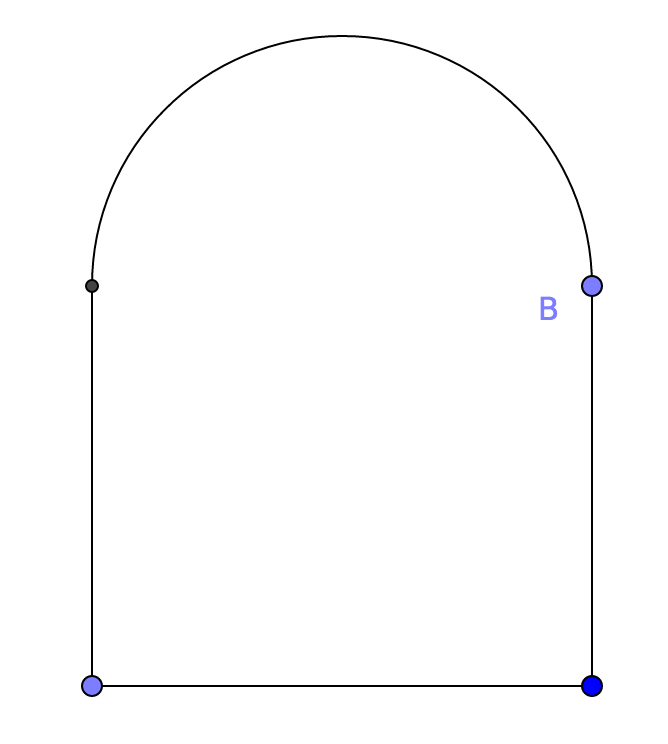
\includegraphics[scale=0.5]{1}
\centering 
\end{figure}

\noindent 3. ?


\newpage
\subsection{} \noindent\fbox{
\parbox{\linewidth}{
Soit $C$ un convexe compact de $\mathbb R^n$. 
\begin{enumerate}
\item Pour $a\in \mathbb R^n\setminus \{0\}$ on considère $\varphi:C\to \mathbb R, x\mapsto 2\langle a,x\rangle$. Montrer que $\varphi$ admet un maximum sur $C$ atteint en un point $x_0$.
\item Soit $H_a=\{x\in \mathbb R^n|\; \langle a,x\rangle=\langle a,x_0\rangle \}$. Montrer que $H_a\cap C$ est un convexe non vide.
\end{enumerate}
}}\\ 
\\ 
\\
\noindent 1. $\varphi$ est continue sur $\mathbb R^n$ (car linéaire à partir d'un espace de dimension finie), donc elle admet un maximum sur le compact $C$.\newline 
2. $H_a$ contient $x_0$. Montrons que $H_a$ est convexe. Soit $x,y\in H_a$ et $\lambda\in [0,1]$. Alors $\langle a,\lambda x +(1-\lambda)y\rangle = \lambda \langle a,x\rangle + (1-\lambda) \langle a,y\rangle = \lambda \langle a,x_0\rangle + (1-\lambda) \langle a,x_0\rangle = \langle a,x_0\rangle$ donc $\lambda x +(1-\lambda)y\in H_a$ et $H_a$ est convexe.\newline 
$H_a\cap C$ est donc convexe comme intersection de deux convexes et non vide car il contient $x_0$.

\subsection{} \noindent\fbox{
\parbox{\linewidth}{
Soient $H$ un espace de Hilbert et $C$ une partie convexe fermée non vide de $H$.
\begin{enumerate}
\item On considère $f:H\to \mathbb R$ définie par $f(x)=(d(x,C))^2$. Montrer que $f$ est différentiable en tout point et calculer la différentielle de $f$ en un point $x$ de $H$. (On considérera le projecteur $P$ de meilleure approximation sur $C$).
\item Soit $\varphi: H\to \mathbb R$ définie par $\varphi(x)=\langle Ax,x\rangle + \langle f,x\rangle$ où $f\in H$ et $A\in \mathcal L_c(H,H)$ auto-adjointe. Déterminer le gradient de $\varphi$ en $x$.
\end{enumerate}
}}\\ 
\\ 
\\
\noindent 1. On rappelle que la projection sur un convexe fermé d'un Hilbert est unique et on notera $p_C(x)$ le projeté de $x$ sur $C$. On rappelle que $p_C$ est $1$-lipschitzienne. \newline
\newline
Soit $x\in H$ fixé et $h\in H$. On a le développement $$\begin{aligned}
\hspace{-2cm}d(x+h,C)^2 &= \|x+h-p_C(x+h)\|^2 \\
&= \|x-p_C(x)+h+p_C(x)-p_C(x+h)\|^2 \\
&= d(x,C)^2+2\langle x-p_C(x),h\rangle + 2\langle x-p_C(x),p_C(x)-p_C(x+h)\rangle + \|p_C(x)-p_C(x+h)+h\|^2\\
&= d(x,C)^2+2\langle x-p_C(x),h\rangle + 2\langle p_C(x)-p_C(x+h),h+x-p_C(x)\rangle + \|p_C(x)-p_C(x+h)\|^2+\|h\|^2
\end{aligned}
$$
Le candidat naturel pour la différentielle de $f$ en $x$ est donc $h\mapsto 2\langle x-p_C(x),h\rangle$.\newline
Sachant que $p_C$ est $1$-lipschitzienne il facile de montrer que $\|p_C(x)-p_C(x+h)\|^2+\|h\|^2 = o(\|h\|)$.\newline \newline
Cependant il est \textbf{remarquablement difficile} de prouver par des moyens élémentaires que $\langle p_C(x)-p_C(x+h),h+x-p_C(x)\rangle = o(\|h\|)$. (On peut montrer facilement que c'est un $O(\|h\|)$ mais c'est insuffisant).\newline 
\newline
On adopte une approche différente:\newline
\textbf{Lemme}: Soit $f,g_1,g_2:H\to \mathbb R$ trois fonctions différentiables en $x\in H$ avec $U$ un voisinage de $x$ et  $$\forall y\in U, g_1(y)\leq f(y)\leq g_2(y)$$ et $g_1(x)=g_2(x)$. \newline  Alors $dg_1(x)=dg_2(x)$, $f$ est différentiable en $x$ et $df(x)=dg_1(x)$.\newline \newline
\underline{Preuve}: Pour $h\in U-x$ on a $g_1(x+h)\leq g_2(x+h)$. On dispose de deux fonctions $\varepsilon_1$ et $\varepsilon_2:H\to \mathbb R$ nulles et continues en $0$ telles que $$g_1(x)+dg_1(x)(h)+\|h\|\varepsilon_1(h)\leq g_2(x)+dg_2(x)(h)+\|h\|\varepsilon_2(h)$$
ie $$dg_2(x)(h) -dg_1(x)(h) + \|h\|(\varepsilon_2(h) -\varepsilon_1(h)) \geq 0$$
Pour $t>0$ on remplace $h$ par $th$ et on obtient 
$$t(dg_2(x)(h) -dg_1(x)(h)) + t\|h\|(\varepsilon_2(th) -\varepsilon_1(th)) \geq 0$$
En simplifiant par $t$ puis en faisant $t\to 0$,
$$dg_2(x)(h) -dg_1(x)(h) \geq 0$$
En remplaçant $h$ par $-h$ dans la dernière inégalité,
$$dg_2(x)(h) -dg_1(x)(h) \leq 0$$
donc $dg_2(x)(h) =dg_1(x)(h)$, ceci étant vrai pour tout $h\in H$, donc $dg_2(x)=dg_1(x)$.\newline \newline
Posons $dg(x):=dg_1(x)$ et réécrivons l'inégalité $g_1(x+h)\leq f(x+h)\leq g_2(x+h)$:
$$f(x)+dg(x)(h)+\|h\|\varepsilon_1(h) \leq f(x+h) \leq f(x)+dg(x)(h)+\|h\|\varepsilon_2(h)$$ 
donc 
$$ \varepsilon_1(h)\leq \frac{f(x+h)-f(x)-dg(x)(h)}{\|h\|}\leq \varepsilon_2(h)$$
Par encadrement, on a pour $\|h\|\to 0$, $\dfrac{f(x+h)-f(x)-dg(x)(h)}{\|h\|}\to 0 $. \newline
\null \hfill $\square$\\

\noindent Revenons au problème. Soit $x\in H\setminus C$ fixé. Posons $x^*=p_C(x)$, $e=\frac{x-x^*}{\|x-x^*\|}$ et $\mathcal H$ l'hyperplan d'appui en $x^*$ de normale $e$, de sorte que $$\mathcal H=\{y\in H, \langle y,e\rangle = \langle x^*,e\rangle\}$$
\textbf{Lemme}: On note $p_{\mathcal H}$ la projection orthogonale sur $\mathcal H$ (qui est un sev fermé). Soit $y\in \mathcal H^+$ et $z\in \mathcal H^-$. Alors $\|y-p_{\mathcal H}(y)\|\leq \|y-y'\|$.  \newline \newline
\underline{Preuve}: C'est géométriquement évident (faire un dessin). Formellement, comme 
$\begin{aligned}[t]\|y-y'\|^2&=\|y-p_{\mathcal H}(y) + p_{\mathcal H}(y)-y'\|^2 \\
&= \|y-p_{\mathcal H}(y)\|^2 + \|p_{\mathcal H}(y)-y'\|^2 -2\langle y-p_{\mathcal H}(y), y'-p_{\mathcal H}(y)\rangle
\end{aligned}$\newline
il suffit de prouver que $\langle y-p_{\mathcal H}(y), y'-p_{\mathcal H}(y)\rangle \leq 0$ (ce qui est encore une évidence géométrique).\newline
Comme $y-p_{\mathcal H}(y)\in \mathcal H^\bot$ (cf théorème de la projection orthogonale sur un sev fermé), et que $\mathcal H^{\bot}=\operatorname{Vect}(e)$ on peut écrire \newline
$y-p_{\mathcal H}(y) = \lambda e$ d'où $\begin{aligned}[t]\langle y-p_{\mathcal H}(y), e\rangle &= \lambda \|e\|^2=\lambda\\ 
&= \langle y, e\rangle - \langle p_{\mathcal H}(y), e\rangle \\
&\geq \langle x^*, e\rangle - \langle p_{\mathcal H}(y), e\rangle \quad \text{car }y\in \mathcal H^+ \\
&= \langle x^*, e\rangle - \langle x^*, e\rangle \quad \text{car }p_{\mathcal H}(y)\in \mathcal H \\
&= 0 \end{aligned} $\newline 
donc $\lambda \geq 0$.\newline
Finalement, $\begin{aligned}[t] \langle y-p_{\mathcal H}(y), y'-p_{\mathcal H}(y)\rangle &= \lambda \langle e, y'-p_{\mathcal H}(y) \rangle \\
&= \lambda \left( \langle e, y'\rangle - \langle e, p_{\mathcal H}(y) \rangle \right)\\
&\leq \lambda \left( \langle e, x^*\rangle - \langle e, x^* \rangle \right) \; \text{car } \lambda\geq 0,\; z\in \mathcal H^-, \;p_{\mathcal H}(y)\in \mathcal H \\
&= 0
\end{aligned}$\newline
comme souhaité. \null \hfill $\square$\\

\noindent Dans notre problème on dispose d'un voisinage de $x$ noté $U$ tel que $U\subset \mathcal H^+$. Pour $y\in U$, comme $p_C(y)\in C\subset \mathcal  H^-$, le lemme donne $(d(y,\mathcal H))^2\leq (d(y,C))^2$. On a aussi la majoration triviale $(d(y,C))^2\leq \|y-x^*\|^2$. En bref $$(d(y,\mathcal H))^2\leq (d(y,C))^2\leq \|y-x^*\|^2$$
Par ailleurs $(d(y,\mathcal H))^2$ se réécrit simplement $$\langle y-p_{\mathcal H}(y),e\rangle^2  = \langle y-x^*,e\rangle^2 = \langle y-x^*,\frac{x-x^*}{\|x-x^*\|}\rangle^2 $$
D'où l'encadrement $$\underbrace{\langle y-x^*,\frac{x-x^*}{\|x-x^*\|}\rangle^2}_{:= g_1(y)}\leq (d(y,C))^2\leq \underbrace{\|y-x^*\|^2}_{:= g_2(y)}$$
On a bien $g_1(x)=g_2(x)$, $g_1$ différentiable en $x$ et $g_2$ différentiable en $x$ de différentielle $h\mapsto 2\langle h,x-x^* \rangle$ (application linéaire continue par Cauchy-Schwarz).\newline
D'après le lemme, $f$ est différentiable en $x$ de différentielle $h\mapsto 2\langle h,x-x^* \rangle$.\newline \newline
Il reste à traiter le cas où $x\in C$. Il suffit de noter qu'alors $$(d(x+h,C))^2\leq \|(x+h)-x\|^2=\|h\|^2$$
Donc $f$ est différentiable de différentielle nulle.
\newpage
\subsection{} \noindent\fbox{
\parbox{\linewidth}{
Soit $C$ un fermé de $\mathbb R^n$ tel que $\forall x,y \in C,\; ]x,y[\cap C \neq \emptyset$.\newline
Montrer que $C$ est convexe.
}}\\ 
\\ 
\\
\noindent Supposons par l'absurde que $C$ n'est pas convexe: on dispose alors de $x,y\in C$ et $\alpha\in ]0,1[$ tel que $(1-\alpha)x+\alpha y\notin C$.\newline\newline 
Considérons $\mu=\inf\{\lambda\geq \alpha| (1-\lambda)x+\lambda y\in C\} $ . On dispose de $\lambda_n$ une suite qui décroit vers $\mu$ avec pour tout $n$, $(1-\lambda_n)x+\lambda_n y\in C$ et $\lambda_n\geq \alpha$. En passant à la limite, comme $C$ est fermé, on a $(1-\mu)x+\mu y\in C$ et $\mu\geq \alpha$. Comme $(1-\alpha)x+\alpha y\notin C$, l'inégalité est stricte: $\mu>\alpha$ .\newline \newline
De même, on pose $\nu=\sup\{\lambda\leq \alpha| (1-\lambda)x+\lambda y\in C\} $. On a encore $(1-\nu)x+\nu y\in C$ et $\nu< \alpha$.\newline \newline
Posons $a=(1-\mu)x+\mu y$ et $b=(1-\nu)x+\nu y$. Alors $]a,b[\cap C\neq \emptyset$: on dispose de $\gamma\in ]0,1[$ tel que $(1-\gamma)b+\gamma a\in C$. \newline \newline
Or $(1-\gamma)b+\gamma a = (1-[(1-\gamma)\nu + \gamma \mu])x + [(1-\gamma)\nu + \gamma \mu]y\;$ avec $$(1-\gamma)\nu + \gamma \mu\in \; ]\nu,\mu[ 
$$
Ceci contredit la définition de $\nu$, absurde.


\end{document}